\documentclass[a4paper]{article}
\usepackage[utf8]{inputenc}
\usepackage{minted}
\usepackage[lang=fortran, verbose, print=m]{fortex}
\usepackage{amsmath, amssymb, amsfonts}
\usepackage[scale=0.9]{sourcecodepro}
\usepackage{microtype}
\usepackage{multirow}
\usepackage{tikz}
\usepackage{graphics}
\usepackage{cite}
\usepackage{imakeidx}
\usepackage{bookmark}
\usepackage{geometry}

\makeindex

\usetikzlibrary{matrix}

\definecolor{fortexbg}{HTML}{F8F8F0}
\usemintedstyle{ayu}
\setfortex{tabsize=2, breaksymbol=\scriptsize{$\hookrightarrow$}, fontsize=\small, breaklines, bgcolor=fortexbg}

% \DefineVerbatimEnvironment{code}{BVerbatim}{baseline=t}

\title{\texttt{writeimg} and an example of Fortex}
\author{Skippi}

\begin{document}

\maketitle{} 

\section{Intro}

Fortex is a language agnostic way of coding in \LaTeX{}. Previous Literate programming tools each have their own strengths and weaknesses. \texttt{CWEB} for example while very powerful and cool, also very complex and quite difficult to learn. On the other side of the coin you have notebooks -- Jupyter and Mathmatica for example. These whilst simple to learn, the notebook has problems with opening in plain text editors and have issues with ``run each cell in tern'' and have no easy language agnosticism. 

Fortex aims to bridge the gap between the two by providing the plain text editing experience and two-way compile from \texttt{WEB} and combine with the easy to use notebook. 

It should be noted that this method is not perfect. You loose some of the expressiveness of \texttt{WEB} and you loose the wysiwyg of notebooks. (Maybe someone in the future could make a wysiwyg frontend).

The aim of this file is to both provide an example. and to provide a use case where graphics make the mathematics make things clearer. As such, there is going to be a bit more detail that would be normal, showing how Fortex can be used.

It should be noted that I do not code as a job and have not studied any CS, I mainly built this to help myself. There are a few outstanding issues with the Fortex \LaTeX{} package, the main one being that line numbering at the moment doesn't work, as I need to find a way to check the line number of the loaded file then overwrite minted's line numbering. I have tried the \texttt{linenos=true, firstnumber=last} options in minted but that still doesn't seem to work.

The second issue is the hard dependency on minted. In reality its not that hard a dependency, because it is only called in 1 place. I am sure listings would work too without the issue of needing \texttt{-shell-esc}, but as of now I am the only user of Fortex. If in the future, people want to add listings support, by all means. 

The final issue is minted needs \texttt{cache=false} due to caches not updating sometimes - not a big deal when its just a little bit of code, but for a lot of code that gets updated frequently, cache invalidation is hard. downside is this makes \LaTeX{} compilation slow.

\section{Write Image}
\label{sec:writeimg}

The aim of the actual code in this module is to provide a way of outputting a Fortran array to disk in image form. There are a few different image libraries out there, but this one aims to be lightweight and dead simple to use. 

I mainly made this library as a way for me to learn Fortran, so there will be bugs and it will not be perfect. I am also using this as a test of my new \LaTeX{} package -- Fortex.

This module provides a few different subroutines and functions, the main one being \texttt{writeimg}, an interface to a handful of subroutines each handling a different code case -- (do you want normalisation or colour). 

This interface writes a .ppm file to the disk.

All of the inputs to the interface remain unmodified, however the function is not without side effects as a large file will be written to disk.

onto the main code
\begin{codeblock}{writeimgf}
\begin{code}
module writeimgf
	implicit none
	private 
	public :: writeimg
	interface writeimg
		module procedure writeimg_mono_nonormal, &
		                 writeimg_mono_normal,   &
		                 writeimg_col_nonormal,  &
		                 writeimg_col_normal
	end interface writeimg

	contains
\end{code}

\subsection{write monochrome image with no normalisation}
\label{sec:writeimgm_nonormal}

This is the subroutine that I end up calling the most from the interface in \autoref{sec:writeimg}. Is it also the simplest, mealy placing the monochrome matrix in each \texttt{R G B} channel of \texttt{writeimgc\_nonormal} in \autoref{sec:writeimg_col_nonormal}.
\begin{codeblock}[noref]{writeimg_mono_nonormal}
\begin{code}
	subroutine writeimg_mono_nonormal(filename, M, sz)
		implicit none
\end{code}

The subroutine signature is shown in the code snippet below, filename should be self explanatory. $w$ and $h$ refer to the size of the matrix and hence the image that you are going to be writing. $M$ is the matrix that you are going to be writing. 

\begin{code}
		character(len = *), intent(in) :: filename
		integer, intent(in) :: sz(2)
		real, intent(in) :: M(:,:)
\end{code}

Finally as mentioned we then pass off to \texttt{writeimgc\_nonormal} by duplicating $M$ into each of the \texttt{R G B} channels.

\begin{code}
		call writeimg_col_nonormal(filename, M, M, M, sz)
	end subroutine writeimg_mono_nonormal
\end{code}
\end{codeblock}

\subsection{write monochrome image}
\label{sec:writeimgm_normal}

This subroutine is the same as the previous -- writing a monochrome matrix to a .ppm file, however instead of the image brightness $A$ being between 
\begin{equation*}
A \in [\min(M), \max(M)]
\end{equation*}
we now explicitly define the range as the 2 components of the \texttt{normal} array.

If the amplitude of the array is greater the provided normalisation, the code will clip the matrix to the boundaries of the range as shown in \autoref{fig:clip}.

\begin{figure}[hbt]
\centering
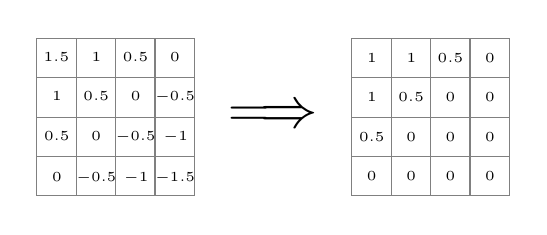
\begin{tikzpicture}[scale=1]
\draw[step=0.5cm, color=gray] (-1,-1) grid (1,1);
\matrix[matrix of nodes,nodes={inner sep=0pt,text width=.5cm,align=center,minimum height=.5cm}]{
\tiny$1.5$ & \tiny$1$    & \tiny$0.5$  & \tiny$0$     \\
\tiny$1$   & \tiny$0.5$  & \tiny$0$    & \tiny$-0.5$  \\
\tiny$0.5$ & \tiny$0$    & \tiny$-0.5$ & \tiny$-1$    \\
\tiny$0$   & \tiny$-0.5$ & \tiny$-1$   & \tiny$-1.5$  \\};

\node at (2,0) {\huge$\Longrightarrow$};

\draw[step=0.5cm, color=gray] (2.999,-1) grid (5,1);
\matrix[matrix of nodes,nodes={inner sep=0pt,text width=.5cm,align=center,minimum height=.5cm}] at (4,0) {
\tiny$1$   & \tiny$1$    & \tiny$0.5$  & \tiny$0$  \\
\tiny$1$   & \tiny$0.5$  & \tiny$0$    & \tiny$0$  \\
\tiny$0.5$ & \tiny$0$    & \tiny$0$    & \tiny$0$  \\
\tiny$0$   & \tiny$0$    & \tiny$0$    & \tiny$0$  \\};

\end{tikzpicture}
\caption{matrix $M$ with amplitude $A$ being clipped to new amplitude $A' \in [0, 1]$}
\label{fig:clip}
\end{figure}

\begin{codeblock}[noindex]{writeimg_mono_normal}
\begin{code}
	subroutine writeimg_mono_normal(filename, M, sz, normal)
		implicit none

		character(len = *), intent(in) :: filename
		integer, intent(in) :: sz(2)
		real, intent(in) :: M(:,:)
		real, intent(in) :: normal(2)
		
		call  writeimg_col_normal(filename, M, M, M, sz, normal)
	end subroutine writeimg_mono_normal
\end{code}
\end{codeblock}

\subsection{write colour image with no normalisation}
\label{sec:writeimg_col_nonormal}

This is the first of the coloured cases. here we are still dealing with the unnormalised case. And we see that unlike \autoref{sec:writeimgm_nonormal}, we are now calculating the normalisation before passing off to \texttt{writeimgc\_normal} in section \autoref{sec:writeimg_col_normal}

As previously mentioned, the normalisation is done by taking the $\min()$ and $\max()$ of the matrices and normalising so everything is in range.


\index{Normalisation}
\begin{codeblock}{writeimg_col_nonormal}
\begin{code}
	subroutine writeimg_col_nonormal(filename, r, g, b, sz)
		implicit none
		
		character(len = *), intent(in) :: filename
		integer, intent(in) :: sz(2)
		real, intent(in) :: r(:,:), g(:,:), b(:,:)
		
		real :: normal(2)
		
		normal(1) = min(min(minval(r), minval(g)), minval(b))
		normal(2) = max(max(maxval(r), maxval(g)), maxval(b))
		
		call  writeimg_col_normal(filename, r, g, b, sz, normal)
	end subroutine writeimg_col_nonormal
\end{code}
\end{codeblock}

\subsection{write colour image}
\label{sec:writeimg_col_normal}

This is the final subroutine that all the above subroutines in \autoref{sec:writeimgm_nonormal}, \ref{sec:writeimgm_normal} and \ref{sec:writeimg_col_nonormal}, eventually filter down too. This handles the saving of the image, the setting of magic header bytes, basically everything.

\begin{codeblock}{writeimg_col_normal}
\begin{code}
	subroutine writeimg_col_normal(filename, r, g, b, sz, normal)
		implicit none

		character(len = *), intent(in) :: filename
		integer, intent(in) :: sz(2)
		real, intent(in) :: r(:,:), g(:,:), b(:,:)
		real, intent(in) :: normal(2)
\end{code}

local variables need to be declared. $i,j$ are loop variables, $r_\text{int}, g_\text{int}, b_\text{int}$ are temporary arrays of integers due to the .ppm fomat using ints and not reals. 

\begin{code}
		integer i,j
		
		integer :: rint(sz(1), sz(2))
		integer :: gint(sz(1), sz(2))
		integer :: bint(sz(1), sz(2))
		
		open(10, file=filename, status='replace', action="write") 
\end{code}

the .ppm format deals with either 8 or 16 bit integers, we need to convert our reals to integers in that range. Here we are using 8 bit images due to the space inefficiency of the .ppm file format. This conversion will be lossy and involve rounding, however if you have a human eye that can tell the brightness difference between $A=123$ and $A=124$, I will be \emph{very} surprised.

The formula for conversion to is given in \ref{eqn:norm} normalises each \texttt{R, G, B} component to $A\in[0,1]$.

\begin{equation}
A_\text{norm} = \frac{A - \min}{\max}
 \label{eqn:norm}
\end{equation}

From here, each component is multiplied by 255 and then rounded to the nearest integer.

\index{Rounding}
\begin{code}
		rint = int( (r - normal(1)) / normal(2) * 255 )
		gint = int( (g - normal(1)) / normal(2) * 255 )
		bint = int( (b - normal(1)) / normal(2) * 255 )
\end{code}

The following code snippet shows the  Magic number for a .ppm file. Other Magic numbers include:

\begin{table}[hbt]
\centering
 \begin{tabular}{|c|c|l|}\hline
	\multicolumn{2}{|c|}{Magic} & \multirow{2}{*}{Colour Range} \\\cline{1-2}
	ASCII & Binary & \\\hline 
	P1 & P4 & Black \emph{or} white (binary) \\\hline
	P2 & P5 & Greyscale $A\in[0,2^8]$ or $A\in[0, 2^{16}]$\\\hline
	\multirow{2}{*}{P3} & \multirow{2}{*}{P6} & Colour $A\in[0,2^8]$ for each channel \\
	& & Support for 16 bit is sketchy\\\hline
 \end{tabular}
 \caption{Magic numbers for .ppm files\cite{davidsennetpbm}.}
\end{table}

Here we are using \texttt{"P6"} due to its colour support and the space savings you get for using binary numbers.

The Magic number is then followed by a newline, the width (in \textsc{ascii}), newline, the height (in \textsc{ascii}), newline, the range (in \textsc{ascii}).
\index{PPM magic}
\begin{code}
		write(10, '(A2)') "P6"
		write(10, '(I0)') sz(1)
		write(10, '(I0)') sz(2)
		write(10, '(I0)') 255
\end{code}

Finally we get to writing the actual image. The image is supposed to be written as one long stream of binary. as such we convert the integers to achars and then write, making sure to suppress automatic newlines.

We write the code in a simple loop as it is the simplest way to interleave the 3 colours. This will however not be cache efficient, but the main bottleneck here is writing the file to disk anyway. These images get large real fast due to no compression and it's very easy to write 200MiB files to disk.
% \vindex|write *,*|
\index{Write image to file}
\begin{code}
		do j = 1,sz(2)
			do i = 1,sz(1)
				write(10, '(A1)', advance='no') achar(rint(i, j))
				write(10, '(A1)', advance='no') achar(gint(i, j))
				write(10, '(A1)', advance='no') achar(bint(i, j))
			end do
		end do
\end{code}

Finally a bit of cleanup

\begin{code}
		close(10)
	end subroutine writeimg_col_normal
end module writeimgf
\end{code}
\end{codeblock}
\end{codeblock}

\bibliographystyle{IEEEtran}
\bibliography{test}
\printindex

\end{document}
